\part{String types}
\frame{\partpage}

\begin{frame}{Strings}
	\begin{itemize}
		\pause\item A \textbf{string} represents a sequence of textual characters
		\pause\item E.g.\ \lstinline{"Hello world!"}
		\pause\item Python type: \lstinline{str}
	\end{itemize}
\end{frame}

\begin{frame}{String representation}
	\begin{itemize}
		\pause\item Stored as sequences of \textbf{characters} encoded as \textbf{integers}
		\pause\item Often \textbf{null-terminated}
			\begin{itemize}
				\pause\item Character number 0 signifies the end of the string
			\end{itemize}
	\end{itemize}
\end{frame}

\begin{frame}{What is a character?}
	\begin{itemize}
		\pause\item Broadly speaking, a single \textbf{printable symbol}
		\pause\item There are also some special \textbf{non-printable characters} e.g.\ line break
	\end{itemize}
\end{frame}

\begin{frame}{ASCII}
	\begin{itemize}
		\pause\item American Standard Code for Information Interchange
		\pause\item Defines a standard set of 128 characters (7 bits per character)
		\pause\item Originally developed in the 1960s for teletype machines, but survives in computing to this day
		\pause\item 95 printable characters: upper and lower case English alphabet, digits, punctuation
		\pause\item 33 non-printable characters
	\end{itemize}
\end{frame}

{
\setbeamercolor{background canvas}{bg=white}
\begin{frame}[plain]
	\begin{tikzpicture}[remember picture, overlay]
		\node[at=(current page.center)] {
			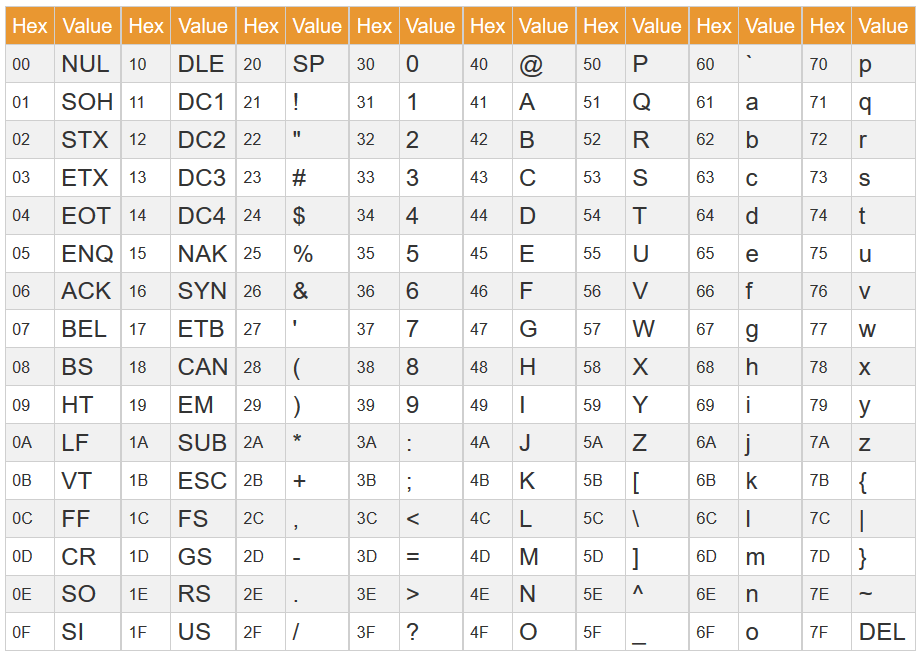
\includegraphics[width=\paperwidth]{ascii_chart_2}
		};
	\end{tikzpicture}
\end{frame}
}

\begin{frame}{ASCII}
	\begin{itemize}
		\pause\item ASCII works OK for English
		\pause\item Standards exist to add another 128 characters (taking us to 8 bits per character)
		\pause\item E.g.\ accented characters for European languages, other Western alphabets e.g. Greek, Cyrillic,
		    mathematical symbols
		\pause\item However 256 characters isn't enough...
	\end{itemize}
\end{frame}

\begin{frame}{Unicode}
	\begin{itemize}
		\pause\item Standard character set developed from 1987 to present day
		\pause\item Currently defines 143859 characters (Unicode 13.0)
		\pause\item First 128 characters are the same as ASCII
		\pause\item Covers most of the world's writing systems
		\pause\item Also covers mathematical symbols and emoji
	\end{itemize}
\end{frame}

\begin{frame}{Encoding Unicode}
    \begin{itemize}
		\pause\item \textbf{UTF-32} encodes characters as 32-bit integers
		\pause\item \textbf{UTF-8} encodes characters as 8, 16, 24 or 32-bit integers
			\begin{itemize}
			    \pause\item 8-bit characters correspond to the first 128 ASCII characters
			        $\implies$ backwards compatible
				\pause\item More common Unicode characters are smaller
				    $\implies$ more efficient than UTF-32
			\end{itemize}
	\end{itemize}
\end{frame}

% \begin{frame}{String representation}
% 	\begin{itemize}
% 		\pause\item \lstinline{"Hello world!"} in ASCII or UTF-8 encoding:
% 	\end{itemize}
	
% 	{\footnotesize\pause\begin{tabular}{*{13}{|c}|}
% 		\hline
% 		72 & 101 & 108 & 108 & 111 & 32 & 119 & 111 & 114 & 108 & 100 & 33 & 0 \\\hline
% 	\end{tabular}}
% \end{frame}

\begin{frame}{UTF-8 representation}
	\begin{itemize}
		\pause\item For characters in ASCII, UTF-8 is the same:
			\begin{itemize}
				\pause\item a $\to [97]$
			\end{itemize}
		\pause\item Other characters are encoded as multi-byte sequences:
			\begin{itemize}
				\pause\item \"u $\to [195, 188]$
				\pause\item 
\includegraphics[height=1.5ex]{chinese}\ $\to [228, 184, 178]$
				\pause\item 
\includegraphics[height=1.5ex]{emoji}\ $\to [240, 159, 152, 130]$
			\end{itemize}
		\pause\item \texttt{"Haha 
\includegraphics[height=1.5ex]{emoji}"} encoded in UTF-8:
	\end{itemize}
	{\footnotesize\pause\begin{tabular}{*{13}{|c}|}
		\hline
		H & a & h & a & space & \multicolumn{4}{c|}{
\includegraphics[height=1.5ex]{emoji}} & null \\\hline
		72 & 97 & 104 & 97 & 32 & 240 & 159 & 152 & 130 & 0 \\\hline
	\end{tabular}}
\end{frame}

% \begin{frame}{Strings in Python}
%     \begin{itemize}
%         \pause\item Python 2 had separate types for ASCII and Unicode strings: \lstinline{str} and \lstinline{unicode}
%         \pause\item Python 3 has just the \lstinline{str} type, which uses Unicode
%         \pause\item String literals are wrapped in \lstinline{'single quotes'} or \lstinline{"double quotes"}
%             (there is no difference)
%     \end{itemize}
% \end{frame}

\begin{frame}[fragile]{Escape sequences}
    \begin{itemize}
        \pause\item Backslash \textbackslash\ has a special meaning in string literals
            --- it denotes the start of an \textbf{escape sequence}
        \pause\item Typically used to write \textbf{non-printable characters}
        \pause\item Most useful: \lstinline{"\n"} is a new line
        \pause\item How to type a backslash character? Use \lstinline{"\\"}
    \end{itemize}
\end{frame}

% \begin{frame}{String literal tricks in Python}
%     \begin{itemize}
%         \pause\item Use triple quotes \lstinline{'''} or \lstinline{"""} for a multi-line string
%         \pause\item Use \lstinline{r" "} or \lstinline{r' '} to turn off escape characters
%             (useful for strings with lots of backslashes, e.g.\ Windows file paths, regular expressions)
%     \end{itemize}
% \end{frame}

\begin{frame}[fragile]{Text files}
    \begin{itemize}
        \pause\item Stored on disk as essentially one long string
        \pause\item Line endings are denoted by non-printable characters
            \begin{itemize}
                \pause\item Unix format: line feed character (ASCII/UTF-8 character 10, \lstinline{"\n"})
                \pause\item Windows format: carriage return character (ASCII/UTF-8 character 13) followed by line feed, \lstinline{"\r\n"}
                \pause\item Most text editors can handle and convert both formats
                \pause\item Most languages allow files to be opened in ``text mode'' which automatically converts
            \end{itemize}
    \end{itemize}
\end{frame}

